\documentclass{sigchi}

% Use this command to override the default ACM copyright statement (e.g. for preprints). 
% Consult the conference website for the camera-ready copyright statement.


%% EXAMPLE BEGIN -- HOW TO OVERRIDE THE DEFAULT COPYRIGHT STRIP -- (July 22, 2013 - Paul Baumann)
%\toappear{Permission to make digital or hard copies of all or part of this work for personal or classroom use is 	granted without fee provided that copies are not made or distributed for profit or commercial advantage and that copies bear this notice and the full citation on the first page. Copyrights for components of this work owned by others than ACM must be honored. Abstracting with credit is permitted. To copy otherwise, or republish, to post on servers or to redistribute to lists, requires prior specific permission and/or a fee. Request permissions from permissions@acm.org. \\
% {\emph{CHI'14}}, April 26--May 1, 2014, Toronto, Canada. \\
% Copyright \copyright~2014 ACM ISBN/14/04...\$15.00. \\
% DOI string from ACM form confirmation}
%% EXAMPLE END -- HOW TO OVERRIDE THE DEFAULT COPYRIGHT STRIP -- (July 22, 2013 - Paul Baumann)
%\toappear{Work in progress. Please do not distribute without express permission of the authors.}


% Arabic page numbers for submission. 
% Remove this line to eliminate page numbers for the camera ready copy
\pagenumbering{arabic}


% Load basic packages
\usepackage{balance}  % to better equalize the last page
\usepackage{graphics} % for EPS, load graphicx instead
\usepackage{times}    % comment if you want LaTeX's default font
\usepackage{url}      % llt: nicely formatted URLs
\usepackage{textcomp}
\usepackage{float}
\usepackage{enumitem}

% llt: Define a global style for URLs, rather that the default one
\makeatletter
\def\url@leostyle{%
  \@ifundefined{selectfont}{\def\UrlFont{\sf}}{\def\UrlFont{\small\bf\ttfamily}}}
\makeatother
\urlstyle{leo}


% To make various LaTeX processors do the right thing with page size.
\def\pprw{8.5in}
\def\pprh{11in}
\special{papersize=\pprw,\pprh}
\setlength{\paperwidth}{\pprw}
\setlength{\paperheight}{\pprh}
\setlength{\pdfpagewidth}{\pprw}
\setlength{\pdfpageheight}{\pprh}

% Make sure hyperref comes last of your loaded packages, 
% to give it a fighting chance of not being over-written, 
% since its job is to redefine many LaTeX commands.
\usepackage[pdftex]{hyperref}
\hypersetup{
pdftitle={Contributing on the Commute},
pdfauthor={LaTeX},
pdfkeywords={public transit, accessibility, crowdsourcing, human values, motivation, value sensitive design},
bookmarksnumbered,
pdfstartview={FitH},
colorlinks,
citecolor=black,
filecolor=black,
linkcolor=black,
urlcolor=black,
breaklinks=true,
}

% create a shortcut to typeset table headings
\newcommand\tabhead[1]{\small\textbf{#1}}

\makeatletter
\let\@copyrightspace\relax
\makeatother

% End of preamble. Here it comes the document.
\begin{document}

\numberofauthors{1}
\author{
  \alignauthor Caitlin Bonnar*, Meg Campbell*, Cynthia Bennett\textsuperscript{\textdagger}, and Alan Borning*\\
    \affaddr{* Dept. of Computer Science and Engineering, University of Washington}\\
    \affaddr{\textsuperscript{\textdagger} Dept. of Human-Centered Design and Engineering, University of Washington}\\
    \affaddr{\{cbonnar, meganca, bennec3, borning\}@cs.washington.edu}
}


\title{ Contributing During the Commute: Why Transit Riders Contribute Information About Bus Stops with StopInfo}

\maketitle

\begin{abstract}
% !TEX root = main.tex

%There are numerous motivations for volunteer contributions to crowdsourced  such as wikis, blogs, open-source software, Citizen Science projects, or Internet forums\cite{moore-2007}. We investigate the values and motivations associated with contributing to Over a nine month period, we collected X information submissions about Y unique bus stops in the greater Seattle area.

We draw upon Value Sensitive Design theory and methodology to investigate community members' motivations for entering landmark information about bus stops through an application called StopInfo. A formative study identified the value of \emph{community} as important to many past and potential StopInfo contributors. We explore this value and others further in second round conceptual and empirical investigations centered around people who have previously contributed stop information to StopInfo, as well as with people who use the app but have never contributed information. Lastly, we evaluate our technology with respect to these values and explore possible designs of StopInfo mechanisms that better support values associated with community. 
\end{abstract}

\category{H.5}{Information Interfaces and Presentation}{User Interfaces}
\category{K.4.2}{Computers and Society}{Social Issues}[Assistive
  technologies for persons with disabilities]

\terms{Design, Human Factors}

\keywords{Public transit, accessible transit stops, community-sourcing, crowdsourcing, human values, motivation, Value Sensitive Design}

% !TEX root = main.tex
\section{Introduction}
\label{sec:intro}



Enabling easy and efficient travel is the goal of many transit information technologies being developed today. Examples of information that these systems might provide include directions from one place to another\footnote{http://maps.google.com}, current traffic conditions\footnote{http://waze.com}, public transit arrival and departure times\footnote{http://onebusaway.org}, or wait time at the airport\footnote{http://gomiflight.com/}. Additionally, since technologies such as smartphones have become more ubiquitous, many applications are now drawing on contributions from travellers using these apps on-the-go to collect information that is localized, descriptive, and up-to-date \cite{harding-2013}. However, ensuring that these benefits are present means that information contributions must not only be accurate, but sustainable. This requires continuing participation from the community, whose motivations for contributing are diverse and may wane over time \cite{moore-2007}.

In this paper, we examine a particular transit information technology called StopInfo. StopInfo provides very detailed information about bus stops with the goal of helping public transit riders, particularly those with visual impairments, find and verify bus stop locations. Preliminary evaluations of StopInfo have shown that it supports independence of blind and low vision transit riders, who reported taking more transit trips with StopInfo than they might have without the tool \cite{campbell-2014}. 

The information presented in StopInfo comes from internal information from a transit agency in the Seattle area augmented with information that is entered by the community, primarily as individuals wait at transit stops. In its first year of deployment, StopInfo has received 1879 user submissions about 1148 unique bus stops in the Seattle area. Due in part to a number of press releases and community outreach events, participation has been relatively well sustained for the first twelve months of deployment. However, as might be expected, the number of new submissions has begun to decline (Figure \ref{fig:submissions}). In order to make sure information is accurate and up-to-date, it is important for StopInfo to support contributors' motivations for continuing to enter information, which may encourage increased or long term participation \cite{reed-2013}.

\begin{figure}[H]
\centering
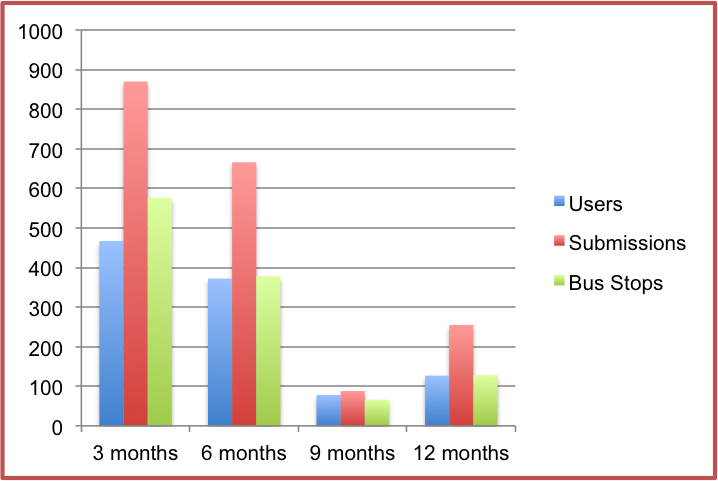
\includegraphics[width=.45\textwidth]{Chart2.png}
\caption{Submission numbers for StopInfo over the first twelve months of deployment. The chart shows the new users, information submissions, and bus stops for each three-month period. We had a major press release occur five months into deployment, and participated in outreach events for StopInfo ten months into deployment.}
\label{fig:submissions}
\end{figure} 


Toward this end, we employ theory and methodology from Value Sensitive Design \cite{friedman-amis-2006} to understand and elicit the values and motivations associated with contributing information about bus stops to StopInfo. In particular, we conduct a survey with previous contributors to the StopInfo system as well as non-contributors (i.e., people who have not contributed to StopInfo before and may or may not be willing to contribute in the future), and are in the process of conducting follow-up interviews with some of these individuals. Early survey and interview results inform us of possible system designs that can potentially help maintain the level of contributions from current StopInfo contributors as well as encourage non-contributors to participate. 





% !TEX root = main.tex
\label{sec:background}
\begin{figure*}[t]
\centering
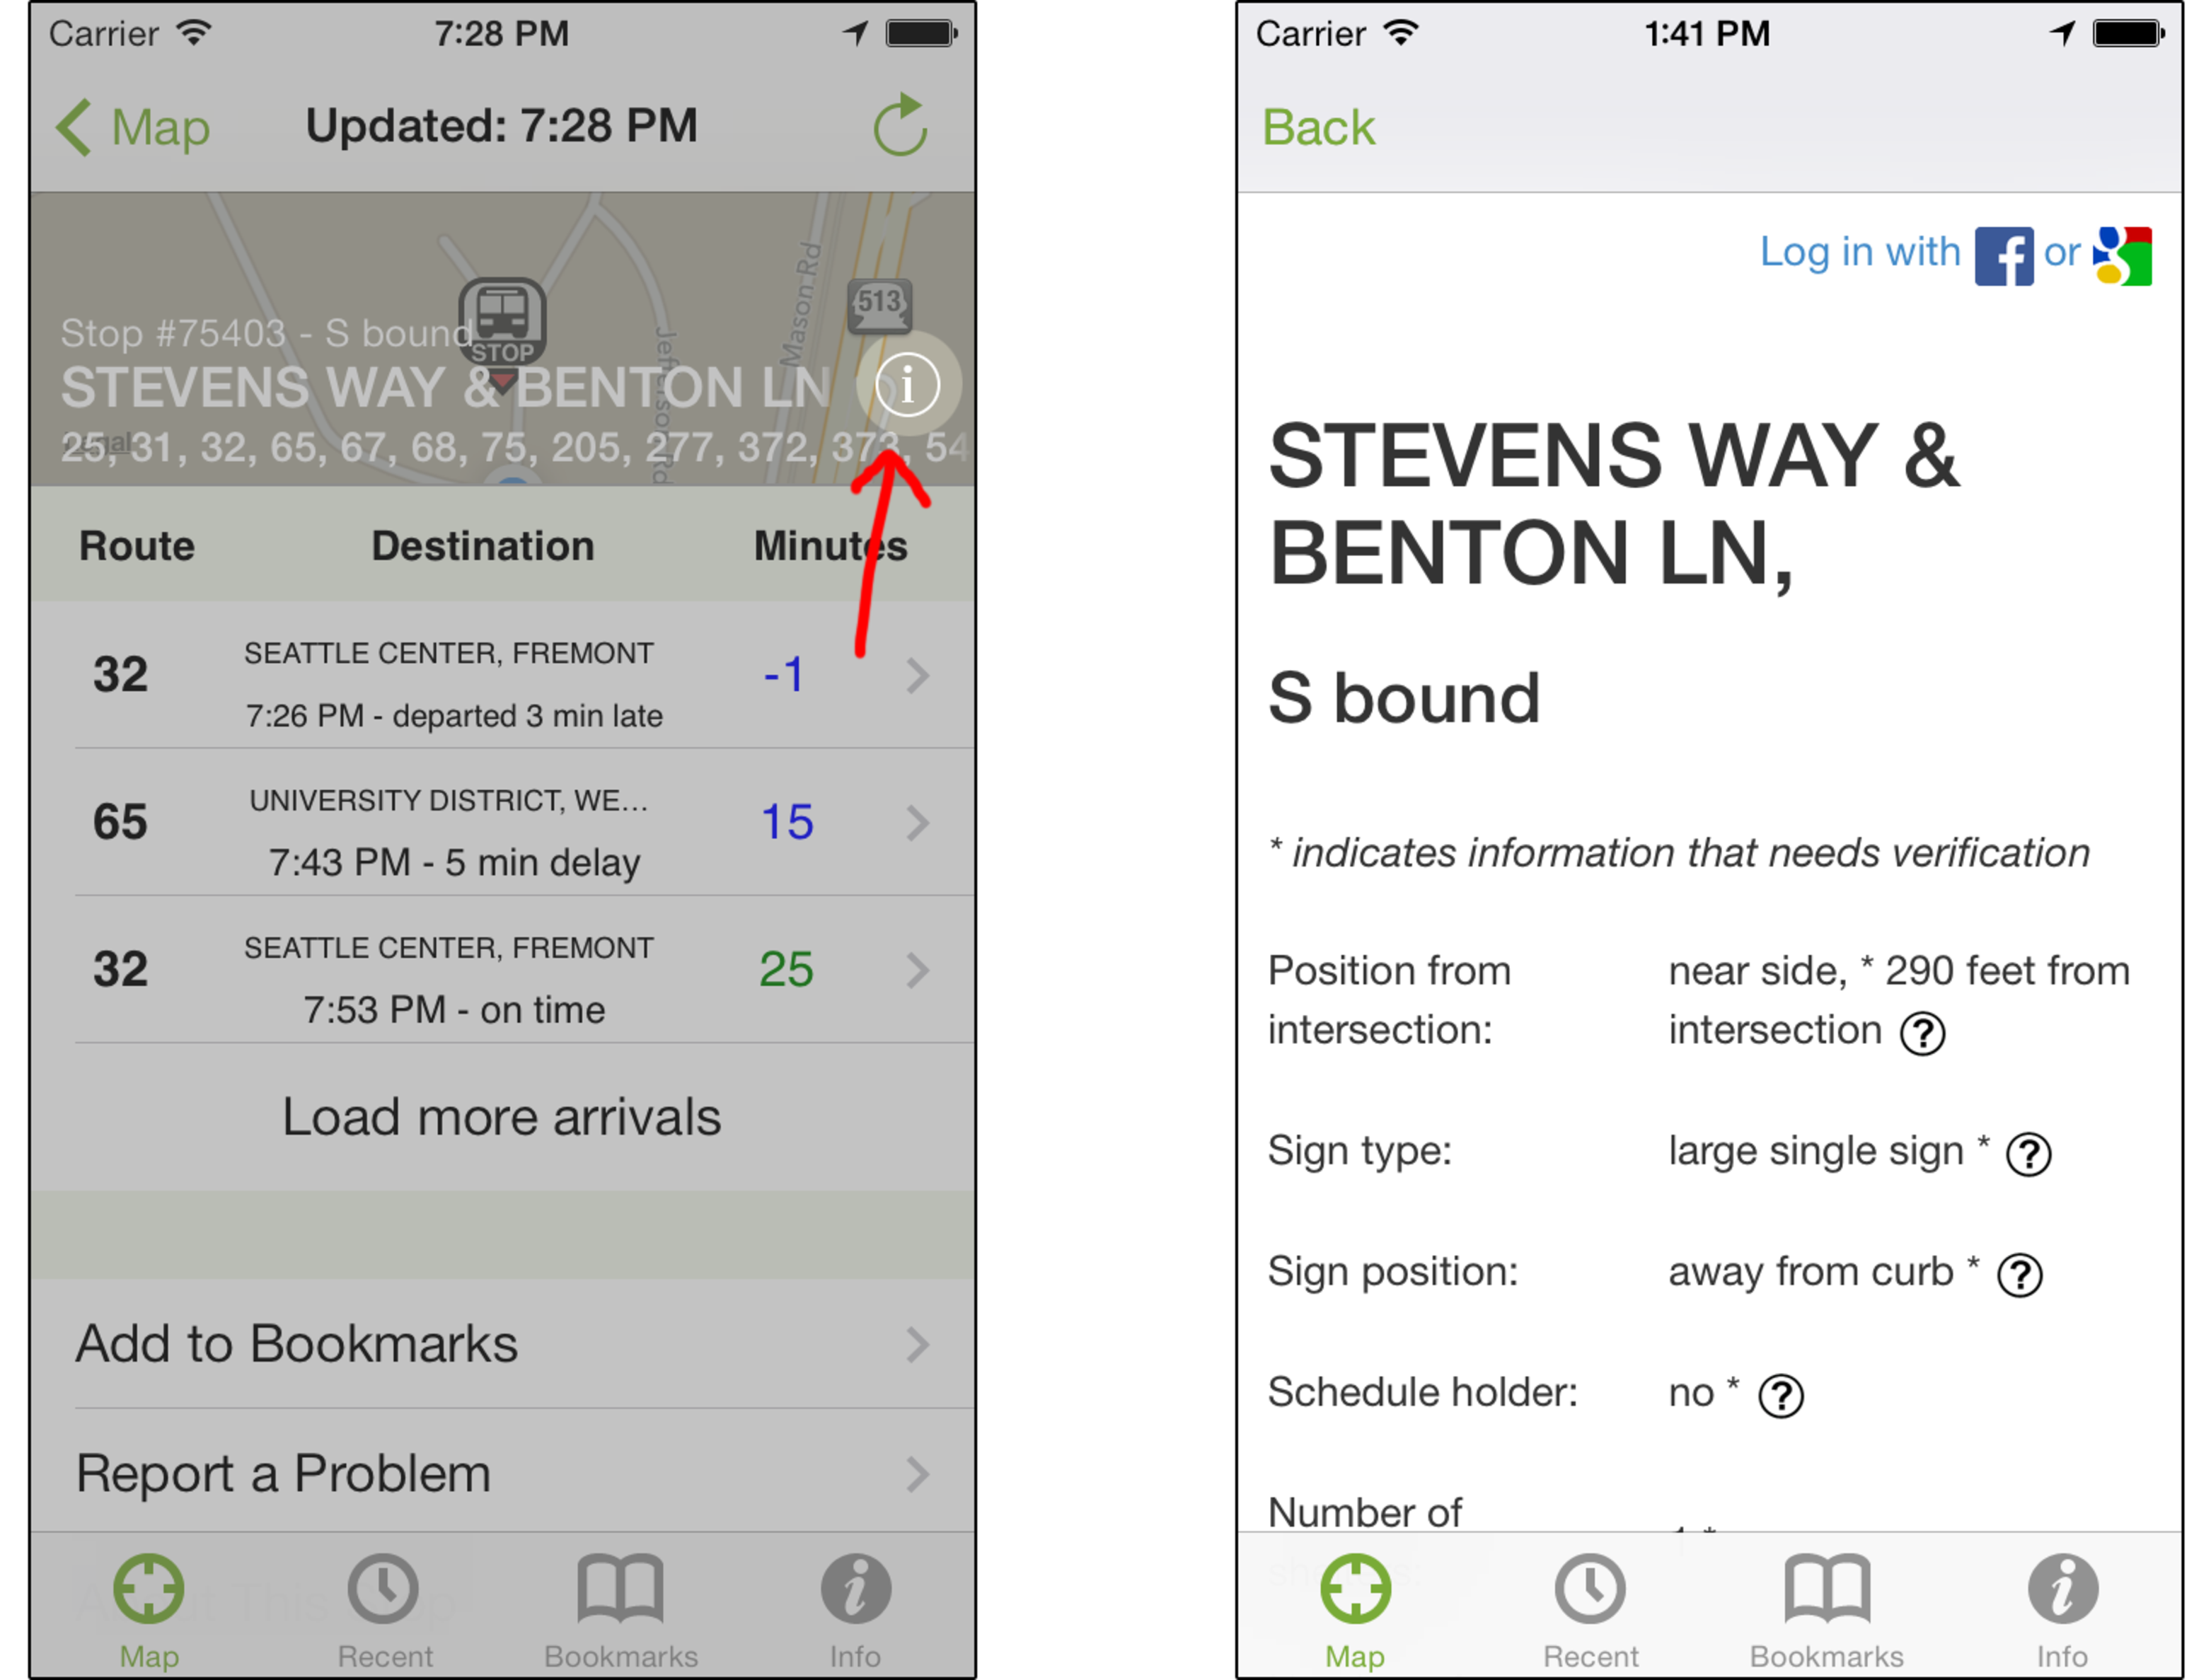
\includegraphics[width=.60\textwidth]{StopInfoAppScreen.pdf}
\caption{(left) The stop details screen in OneBusAway. StopInfo can be
accessed through the info button next to the title. (right) The StopInfo
view and associated information for the specified stop. An asterisk
next to a field means that information has not yet been verified by three 
or more people. If no information exists for a particular field, we do not
display it.  Both screens were also tested extensively for
accessibility using VoiceOver.}
\label{fig:app-screen}
\end{figure*} 

\section{The StopInfo System}

\subsection{OneBusAway}
StopInfo is a web-based application that has been incorporated into OneBusAway \cite{ferris-phd, watkins-phd},
a set of tools that provide real-time arrival
predictions and other transit information, such as where bus stops
are located on a map and which stops are traversed by a particular
route. OneBusAway builds on the work of Dan Dailey and others on real-time transit 
information systems, such as MyBus and BusView \cite{maclean-trb-2002}, and has been widely 
adopted in the Puget Sound region, used by over 100,000 unique transit riders each week. The system is freely available as an application on the iOS, Android, and 
Windows Phone platforms, and also via SMS, interactive voice response, and the 
Web. Research on OneBusAway has found a number of significant 
benefits, including increased or greatly increased satisfaction with public 
transit for 92\% of survey respondents, increased feelings of safety for some
(particularly while waiting at night), and decreased wait time at the stop
\cite{watkins-transportation-research-2011}.  One of the goals of our research 
group is to make these benefits available to as wide a range of people 
as possible, and we have devoted significant attention to ensuring that the
apps, in particular the iOS app, provide adequate accessibility.

We decided to integrate StopInfo with OneBusAway on iOS for a number
of reasons. First, OneBusAway is already used by a large number of
people, and many check the application from their smartphones while 
waiting at bus stops. This enables us to leverage a large existing user base by directly allowing the community to enter information for the stop as they 
wait. Secondly, the OneBusAway iOS application is already heavily used 
by members of the blind, low vision, and 
deaf-blind communities in the greater Seattle region who use and rely on
public transit, and has been developed and tested to remain
accessible to this community. Finally, StopInfo is a natural extension of 
OneBusAway, and can also be useful to
the general population of transit riders. It includes relevant information such 
as how well-lit a stop is at night, which has safety implications, and whether
a stop may be closed.

We integrated StopInfo with OneBusAway iOS by placing an info button with the
accessibility label ``About This Stop'' next to the name of the stop on the 
details view for that stop (Figure \ref{fig:app-screen}).  Tapping or double tapping 
on the button brings up StopInfo as an integrated
web view within the application, and is also accessible to people with visual impairments through Apple's
VoiceOver screen reader. 

\pagebreak

\subsection{StopInfo Interface}
When a user accesses StopInfo, they are presented with a text list of the stop features.  
An asterisk next an item of information indicates that the information still needs verification from at least two more people.

Below the list of stop information there are links to add or verify information,
report a stop closure, or access some frequently asked questions. In the top right corner of the screen, there is an option to sign in with an existing Facebook or Google account. 

To help encourage contributions, five months after our initial launch of StopInfo, we introduced a reputation system that allows users who are signed in to earn points and badges by entering stop information. They can also make it onto a ``top contributors'' list if they choose to display their profile publicly and if they are among the top twenty users points-wise. For a short time, we also offered the top information contributors free bus passes provided by King County Metro as potential rewards. 

\subsection{Accuracy and Completeness of Information in StopInfo}

In an initial audit conducted two to three months into the deployment of StopInfo, we found that the information submitted by contributors was largely accurate for most categories (the categories that were less accurate were due to ambiguities on our part, which we have since improved) \cite{campbell-2014}. Another accuracy audit is soon forthcoming, which will inform us of any other potential ambiguities or undesired behaviors in the system (however, we have been manually monitoring submissions and have thus far not noticed malicious or gaming behaviors). 

In terms of completeness, out of the 8,481 total bus stops in our system, we have basic information (the position of stop relative to the intersection, the number of shelters, and the type of sign) for all of them, since it was provided by King County Metro. Additionally, StopInfo contributors have added information for categories not provided by the transit agency for 1,148 stops (or 13.5\% of the total stops covered by King County Metro). Each of these stops received one to two submissions on average (of course, some have many more submissions depending on how frequently that stop is accessed). While we are happy with that number, we believe we can do better in terms of breadth by incentivizing people to contribute to stops they do not normally frequent (or extending access and awareness of StopInfo to certain areas). Possible incentives for encouraging breadth will be discussed in a later section.

% !TEX root = main.tex
\section{Value Sensitive Design}
\label{sec:vsd}

Much of our research is ultimately motivated by attempting to better
support certain human values such as independence, safety, equity,
participation, respect, and community.  To approach these value
questions, we employ Value Sensitive Design
\cite{friedman-amis-2006}, a principled, systematic approach to the
consideration of human values in the design of information technology. The primary features of Value Sensitive Design are: consideration of
both direct and indirect stakeholders (that is, the users of
technology and those affected by the technology even though they do
not use it); a tripartite methodology, consisting of conceptual,
empirical, and technical investigations, iteratively and integratively
applied; and an interactional theory to the value implications of
technology.

In other prior Value Sensitive
Design work \cite{borning-ecscw-2005,borning-chi-2012}, the
researchers found it valuable to draw a distinction among stakeholder
values, explicitly supported values, and designer values --- an
important designer value for us is avoiding paternalism toward people
with disabilities.

In the work reported here, we focus on one key set of direct
stakeholders: the information contributors to the StopInfo application. Prior work has investigated values associated with other stakeholders of this application, notably blind and low vision users of StopInfo \cite{campbell-2014}. We also identified general users of StopInfo as direct stakeholders, and bus/train operators, orientation and mobility (O\&M) instructors, King County Metro representatives, and family and friends of blind and low vision users of StopInfo as key indirect stakeholders.

\subsection{Value Scenarios}
Other works utilizing Value Sensitive Design include \emph{value scenarios}, a technique for envisioning the effects of technology designs while in the formative stages of design and value priorities are still unknown \cite{nathan-2007}. Value scenarios are brief fictional descriptions meant to evoke social and value implications associated with a hypothetical technology or feature design. For example, Czeskis et al. use value scenarios to explore the potential impact of a hypothetical mobile location monitoring application on the relationship between parents and their teens \cite{czeskis-2010}.

\pagebreak

\subsection{Value Dams and Flows}
Another methodology introduced in previous work \cite{miller-2007} that we utilize here are Value Dams and Flows. \emph{Value Flows} are defined to be the technical features or organizational policies that a large percentage of stakeholders would like to see included as part of the overall system. Conversely, \emph{Value Dams} refer to the technical features or organizational policies that are strongly opposed, even by a small percentage of stakeholders. Taken together, dams and flows support the desires of the majority and can help alleviate the concerns of minority groups. 


% !TEX root = main.tex
\section{Related Work}
\label{sec:related-work}
As part of the conceptual investigation for uncovering motives and values surrounding information contributors' use of StopInfo, we first explored existing literature to try and identify potential values of interest for our own work.

\subsection{Motives for Contributing}
Much work has been done on investigating motives for contributions to crowdsourcing technologies such as Wikipedia \cite{oreg-2008, schroer-2009}, citizen science projects (e.g. Stardust@home, FoldIt, GalaxyZoo) \cite{eveleigh-2014, nov-2011, prestopnik-2011, reed-2013}, question and answer forums (e.g. Yahoo! Answers \cite{dearman-2010}, Math Overflow \cite{tausczik-2012}), open source projects \cite{oreg-2008, wu-2007}, and other knowledge-sharing systems \cite{miller-2007}. Additionally, Moore et al. investigated how type and purpose of a virtual community (e.g. wikis, blogs, or Internet forums) correlates with members' motives for participating \cite{moore-2007}. 

A system that provides detailed transit stop information can be
viewed as a specialized geowiki.  Literature on geowikis includes 
OpenStreetMap\footnote{http://openstreetmap.org}, which
is certainly the largest geowiki. Haklay
\cite{haklay-environment-planning-b-2010} provides an assessment of
the success of OpenStreetMap, both in terms of accuracy and coverage,
in comparison with Ordnance Survey datasets in the United 
Kingdom. Another notable geowiki is Cyclopath for bicyclists
\cite{panciera-chi-2010,priedhorsky-wikisym-2007},
which also includes route-finding capabilities. However, it is unclear whether motivations for contributing to wikis such as Wikipedia (which is perhaps the most well-studied) extend to geowikis. For example, Moore et al. identify the motives of \emph{altruism}, \emph{belonging}, \emph{collaboration}, \emph{egotism}, \emph{knowledge}, \emph{power}, \emph{reciprocity}, \emph{reputation}, and \emph{self-esteem} as pertaining to wiki participation \cite{moore-2007}. However, a system such as StopInfo or OpenStreetMap requires simple contextual knowledge (i.e., physical features that are present in a specific area) rather than expert knowledge; thus, it is unclear whether motives such as knowledge (in the sense of improving knowledge rather than sharing) or power might apply. 

Based on our present knowledge, contribution behavior and motivations surrounding crowdsourced transit information systems such as Waze or MiFlight are not currently well-studied. Work by Lathia et al. regarding transit riders' experiences with a crowdsourced transit information system for the London Underground called TubeStar mentions studying contributors' motives as future work \cite{lathia-2014}; however, to present, there is little work in this arena. 

\subsection{Reputation and Badge Systems}

Based on prior literature \cite{antin-2011, depaoli-2012, mamykina-2011}, we decided to implement a reputation system as well as a badge system as part of StopInfo. These works have shown that certain game elements, such as earning points and unlocking achievements (i.e., badges), have led to increased participation and have helped sustain contributions over time \cite{iacovides-2013}. Badges can also serve as a representation of \emph{community membership}, \emph{authority}, \emph{competence}, \emph{experience}, \emph{identity}, and \emph{reputation} \cite{halavais-2012}.

% !TEX root = main.tex
\section{StopInfo Contributor Values}
\label{sec:contributor-values}

Our initial work with the StopInfo system focused on the values associated with blind and low vision transit riders, the primary group for which StopInfo was designed \cite{campbell-2014}. However, the system would not be useful to this stakeholder group (or StopInfo users in general) if the information provided is not reliable, meaning that it must be both \emph{accurate} and \emph{complete}, which were discussed in the StopInfo section previously.

To help bolster the completeness and accuracy of StopInfo information, we decided to investigate the motivations and values associated with contributing information to StopInfo with former and potential contributors, in hopes of being able to increase and sustain the level of contributions all the while promoting high-quality submissions.   

\subsection{Formative Study}
During the summer of 2014 (five months after StopInfo had been deployed), we performed a formative study by surveying 15 StopInfo contributors and 31 non-contributors. The survey addressed the basic usability of our current StopInfo system\footnote{At the time, we had just incorporated the top contributor list and badge system, and no one participating in the survey reported having noticed them before, so we do not believe these aspects of the system were well addressed.} and asked about potential motivations for contributing information about bus stops. 

We also spoke to nine participants in follow-up semi-structured interviews about their contributions to other projects that involve crowd or community sourcing, and their views of the StopInfo project as a whole. To us, one of the more interesting findings from this study was the emphasis on wanting to interact with and benefit the community, although it was not clear to us what who was meant by `community' here.

\subsection{Optimal Conditions for Submitting}
From these results, we also learned what might entail optimal (i.e. lowest cost) conditions for contributing information to StopInfo. That is, intrinsic motivating factors and incentives aside, StopInfo contributors and non-contributors alike reported that they would be most \emph{able} to contribute to StopInfo if:
\begin{itemize}[leftmargin=8mm]
\item It is easy enough to get to StopInfo within the OneBusAway application.
\item They are aware of the presence of StopInfo while waiting at a bus stop.
\item They have downtime while waiting for their bus.
\item The form is quick to fill out and the categories of information are unambiguous.
\end{itemize}

The above cases mostly center around system usability, opportunity to enter information, and salience. In terms of conditions that we can directly impact, we are continually working to improve the salience and ease of access of the StopInfo feature within OneBusAway, as well as highlight the option to edit stop information while the individual is viewing that stop's information page. Outside of the system itself, we are also participating in outreach (e.g., attending relevant events and sending out press releases). We would also like to put up physical notices (along with Braille translations) at bus stops around Seattle to call attention to the StopInfo feature.

\subsection{Incentivizing Higher Cost Submissions}

Additionally, we learned that some contributors would be willing to submit information at a higher cost given enough incentive and/or intrinsic motivation. Cases in which the cost for submitting information would be higher for contributors include (but are not limited to):
\begin{itemize}[leftmargin=8mm]
\item Going out of their way to visit a stop that is in need of information.
\item Memorizing or taking pictures of stop features to later fill out an information form for that stop.
\item Submitting information even though they find it boring.
\end{itemize}

To mitigate some of these costs, we can work to enhance ease of use within the system itself (for example, by letting users take pictures of the stop directly from the app, or highlighting which stops are in need information on the map), bolster the motivations of those who are willing to put up with a higher cost (such as showing them the direct impact of their submission), or add further incentives (such as a badge that rewards breadth of contribution, monetary or physical rewards, or an optional scavenger-hunt-like game). However, our formative study did not investigate whether people would a) be responsive to these types of features, or b) if they would potentially encourage undesired behaviors, such as gaming the system for rewards. 

\subsection{Value Scenario for StopInfo}
Based on the conditions for submitting outlined above, we decided to compose a value scenario in order to highlight some of the values and potential uses (and misuses) of the system implicated by adding incentives (such as a game) to the system. 

\subsubsection{Value Scenario: Exploring the City with StopInfo}
Growing up, Lisa has always enjoyed solving puzzles and going on scavenger hunts. Over the past year since she's moved to Seattle, she has gotten really into the geocaching\footnote{https://geocaching.com/} phenomenon with her friends. She's found hidden geocaching tags while on hikes, exploring landmarks downtown, and dining at some of the city's local restaurants. Lisa regularly takes the bus to explore these new destinations, and when she learns that the StopInfo system now has a geocaching-like game for some of the bus stops in the Seattle area, she is excited to play along, since now her explorations will also benefit others in the Seattle community. She begins to routinely visit new stops in order to try and find `tagged' stops by entering information in StopInfo for those stops. She becomes a top scorer in the system, and she and her friend Andrew routinely battle for a higher ranking.

A few months later, Lisa twists her ankle while playing soccer and is forced to use crutches for a few weeks. Now, exploring stops that are out of her way is much more of a hassle, and in some of the hillier parts of Seattle, virtually impossible. Andrew zooms past her in the rankings, sending a few gloating messages her way. The competitive side of Lisa is fired up, and she decides to resort to other methods to `explore' new stops. She first uses Google Street View to look at pictures of far off stops and enters information in StopInfo that way. She starts uncovering hidden tags in no time, regaining her footing over Andrew, and wonders why she didn't think of doing this in the first place.

Andrew becomes suspicious of all of Lisa's activity given her injury and visits one of the stops she has entered information for recently. He notices the information she entered is mostly accurate, but that she had entered information for the wrong type of sign. When he accuses Lisa of cheating, she confesses that she used Google Street View to fill in the information. He sighs and tells her those photos are at least a year old, and the sign must have since been replaced for that stop. This kills the honest fun of the game between the two, and they begin to trust the information that other contributors have entered much less. 

\subsubsection{Discussion of Value Scenario}
This scenario highlights the motivating power that games such as geocaching hold in addition to some of the potential pitfalls. In the scenario, Lisa and Andrew both start playing the game to have fun, explore new areas, and benefit others who are using the system. However, as they start to get more competitive, Lisa resorts to gaming the system in what she does not think is a harmful manner. She loses sight of the purpose of the game in order to `beat' Andrew, and ends up submitting less accurate information as a result. This ends up undermining the whole system for the two of them, as well as the end users who experience the inaccurate information, and perhaps also other StopInfo contributors who detect the gaming of the system.

Without ample accurate information as a baseline, it would be difficult to monitor all submissions of information from people playing the game. In this scenario, we can see that competition can sometimes lead to inaccurate submissions, whether the intent is malicious or not. Designing a game like the one described above would have to be done with great caution to make sure that the quality of submissions does not suffer as a result. Furthermore, merely the inclusion of a game in general can potentially undermine submissions from those who are not interested in competition and/or incentives and just want to submit information for more altruistic reasons. 

\subsection{Harms and Benefits Analysis}

For the next phase of our conceptual analysis, we utilized another method associated with Value Sensitive Design: the identification of harms and benefits associated with the StopInfo system for StopInfo contributors. To conduct this analysis, we utilized the findings from our literature review on other contribution-based systems similar to StopInfo, the results from our formative empirical study, the value scenario about gamification of the system, and the informal feedback we have received from the community through outreach events and e-mail. We wished to systematically consider different potential designs of the StopInfo system in order to evaluate harms and benefits associated with the inclusion or omission of particular features, such as the top contributor list, a forced sign-in, or a request system. The designs we evaluated are presented below:

\begin{enumerate}[leftmargin=8mm]
\item Original StopInfo design (can choose to sign in but not required, only a display name and e-mail address collected with signed in; no identification of stops that need information; no badges, points, or top contributor list)
\item Orig. design + reputation system (addition of top contributor list and points earned for certain behaviors, forced to sign in with Facebook or Google account to participate)
\item Orig. design + badge system (addition of badges that can be earned for certain behaviors, do not need to sign in to earn)
\item Orig. design + anonymous request system (identification of specific requests from StopInfo users, requester and responded both anonymous)
\item Orig. design + blind/low-vision request system (identification of specific requests from StopInfo users, where requester can optionally self-identify as blind or low vision)
\item Orig. design + personal request system (identification of specific requests from StopInfo users, where requester and responder must sign in and both can view display name and/or pictures) 
\item Orig. design + optional game (support for a geocache-like game that incentivizes traveling to particular stops to search for clues)
\end{enumerate}

After we listed the potential benefits and harms associated with each system for StopInfo contributors, we mapped them to underlying values. For example, some of the values associated with the addition of the reputation system described in \#2 above included recognition (both from the us, the system administrators, and by other StopInfo users), reputation (in the Seattle community or within the system itself), self-esteem, and privacy. Other potential values implicated by StopInfo include self-efficacy (the feeling that your contributions are useful), safety (in this case, physical well-being), entertainment, and community, which we further break down into \emph{belonging to community} (feeling that you are a part of a group or collective identity), and \emph{concern for community} (or altruism). 


\subsection{Empirical Analysis of StopInfo Contributor Values}

After we completed our conceptual analysis for StopInfo contributors, we decided to do an empirical investigation in order to evaluate our list of values, determine value priorities, and highlight potential value tensions that might arise within the StopInfo contributor stakeholder group itself or with other groups, such as the blind and low vision users of the system.

\begin{figure}[h]
\centering
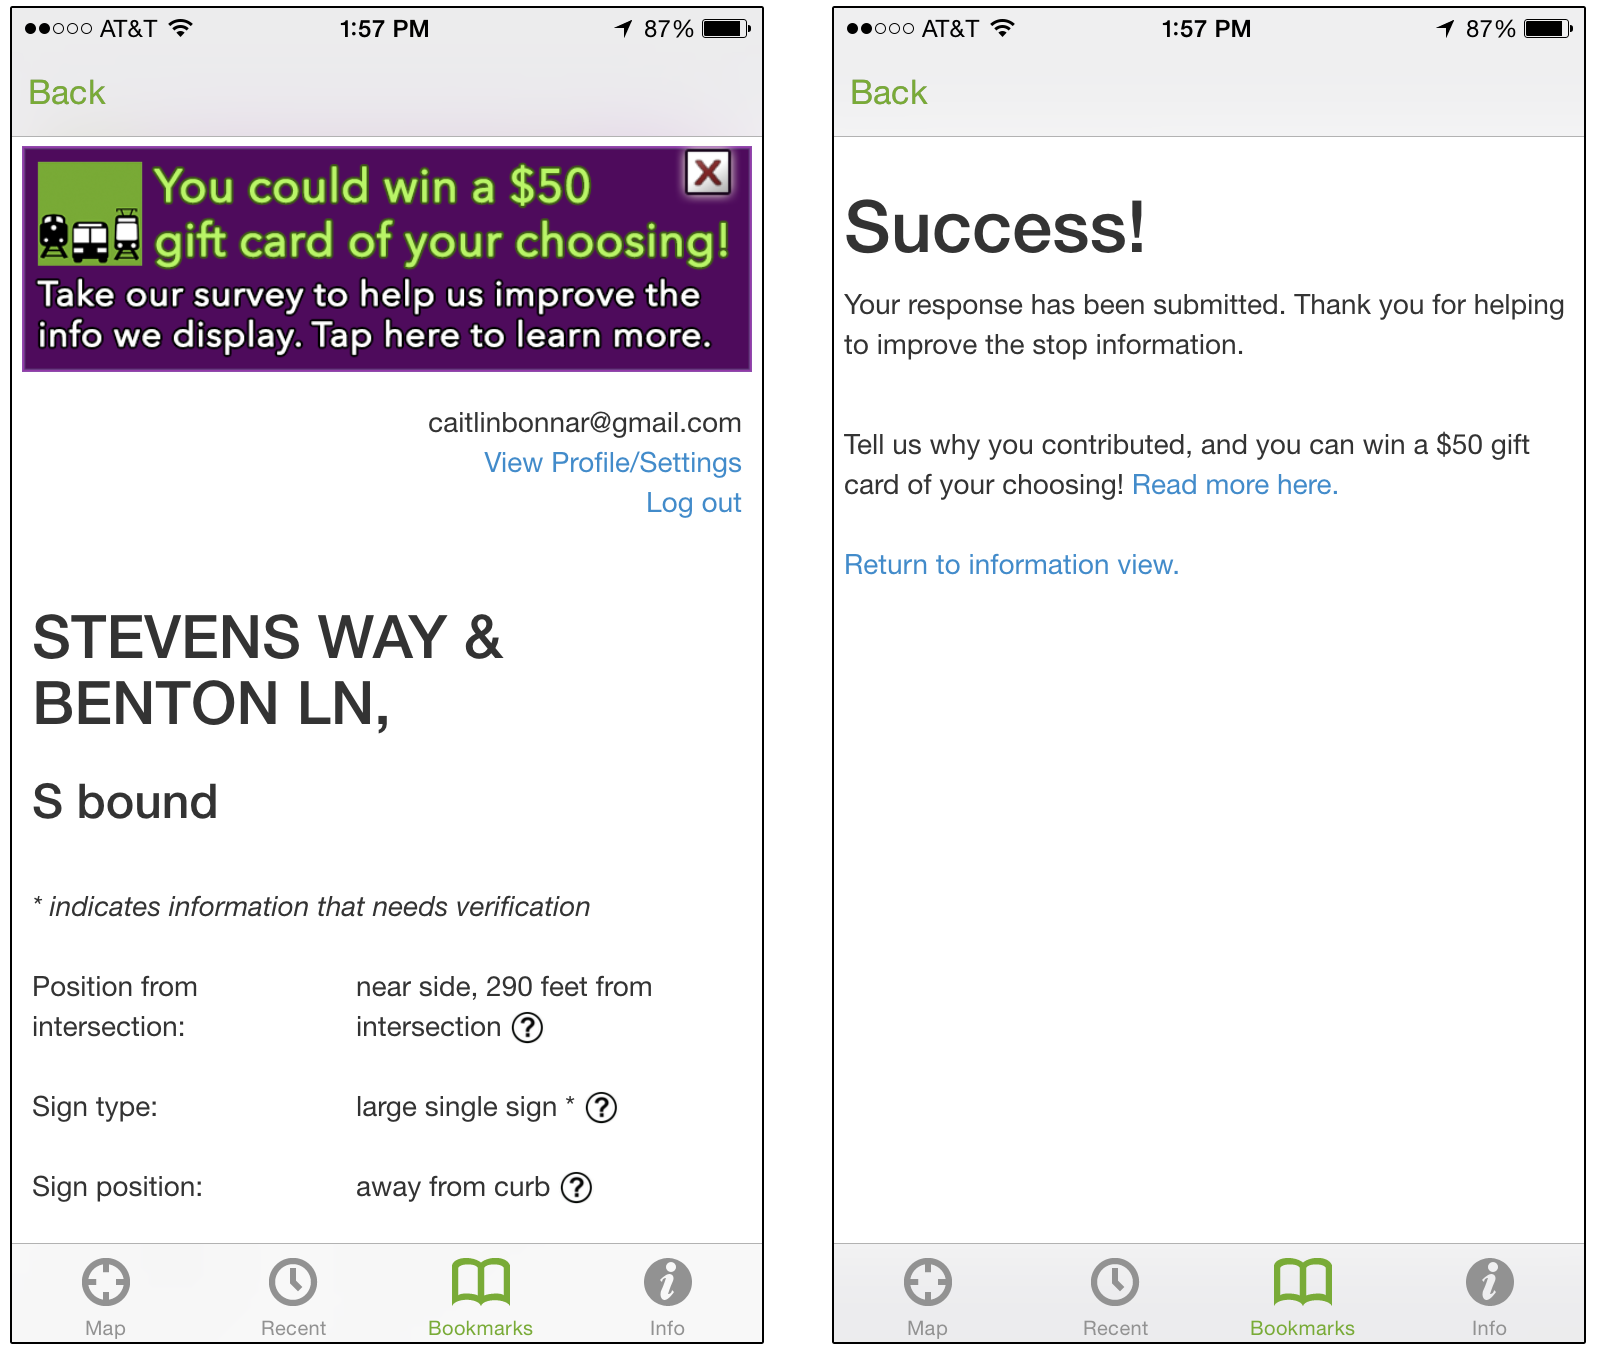
\includegraphics[width=.5\textwidth]{SurveyAlerts.png}
\caption{Screenshots of the survey recruiting methods we placed within the StopInfo application itself. The left screenshot includes a banner at the top of a stop's information page that the user can tap on to view the survey URL. The right screenshot includes the message that appears when a user submits information about a stop that also takes them to the survey URL.}
\label{fig:alerts}
\end{figure} 

\subsubsection{On-line Survey}
To begin the empirical investigation we created an on-line survey for both StopInfo contributors and non-contributors (primarily those who are frequent public transit riders and OneBusAway users). The survey includes structured questions based on some of the values identified in the harms and benefits analysis, as well as open-ended questions that allow for unstructured feedback. The survey was laid out as follows (each item corresponds to a different page of the survey):

\begin{enumerate}[leftmargin=8mm]
\item A consent page that informed them of the purpose of our study
\item Questions about public transit and OneBusAway usage
\item An overview of the StopInfo system including screenshots and a link to the live user interface, what information we collect from contributors, and the goal of the project
\item A question asking whether they have previously contributed to StopInfo
\item A list of open-ended questions about their motivations for contributing and concerns with the current system
\item Structured questions (answered on a 5-point Likert scale) about why they might or might NOT contribute 
\item Both structured and unstructured questions about potential new features and designs of the StopInfo system (including what information they would feel comfortable or uncomfortable with being collected or displayed as part of contributing)
\end{enumerate}

\begin{figure*}[t]
\centering
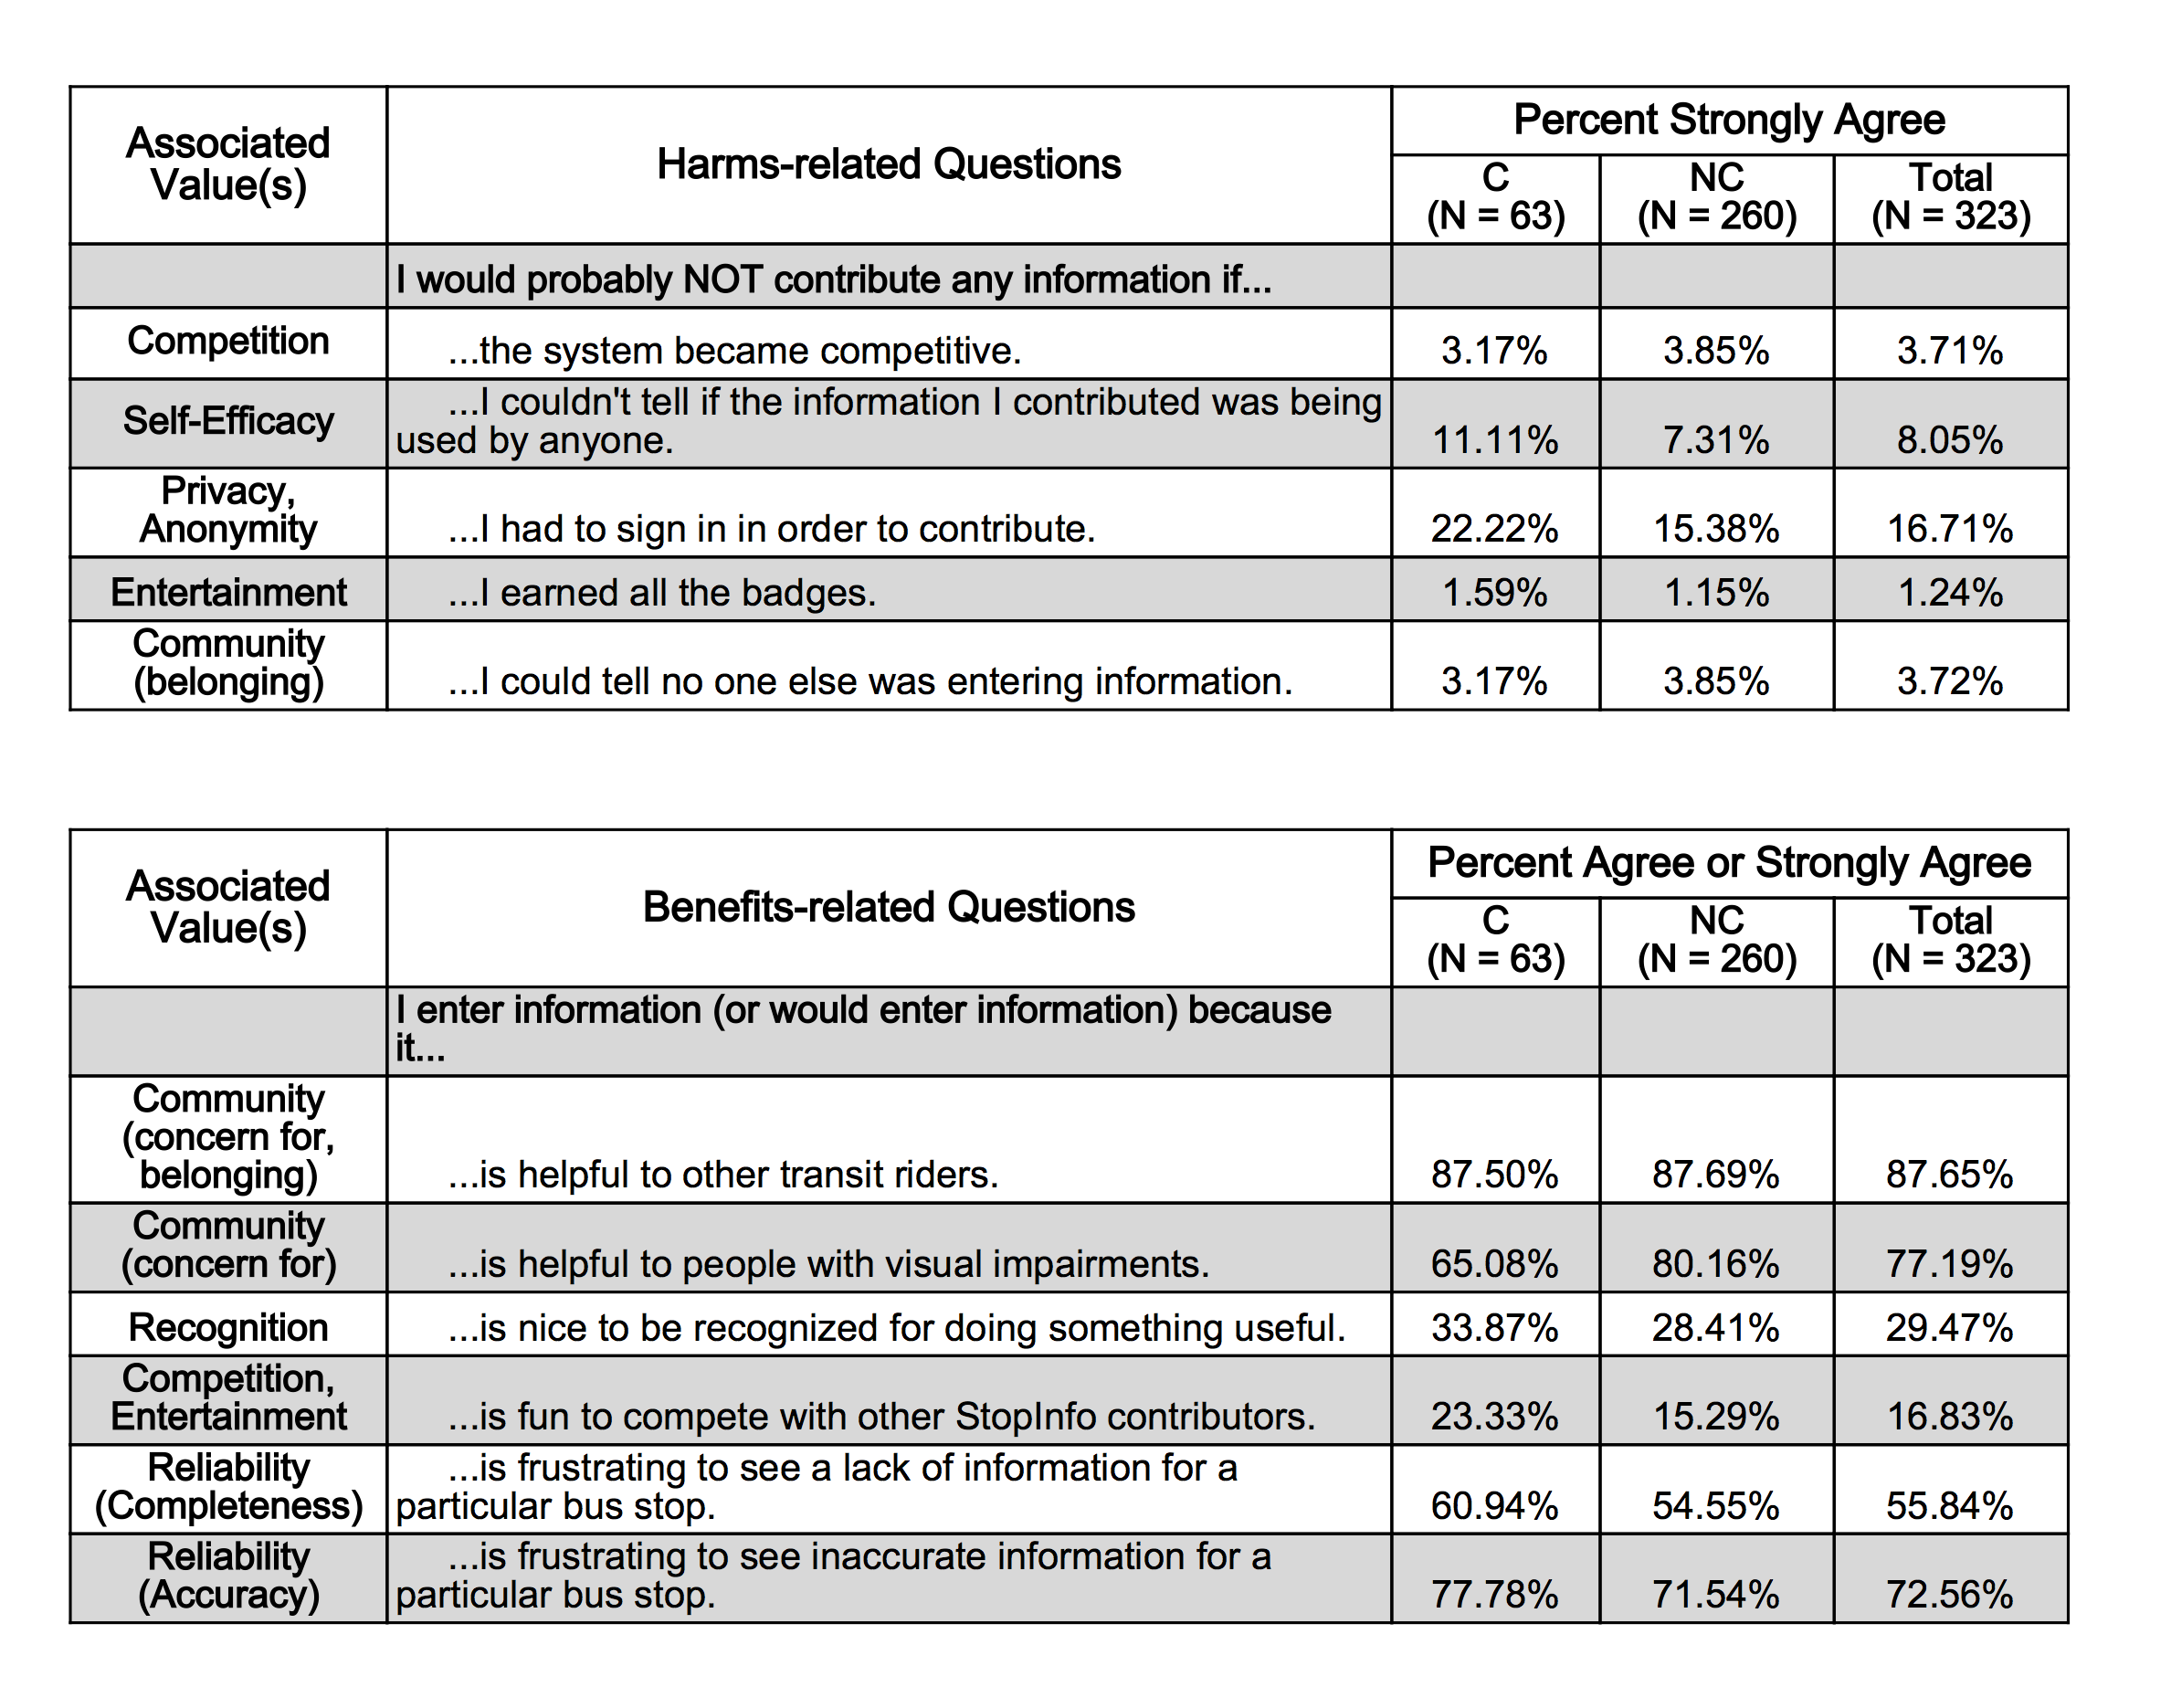
\includegraphics[width=\textwidth]{Results.png}
\caption{Selected preliminary survey results. Here we are considering both previous contributors to the StopInfo system (C, \emph{N} = 63) as well as non-contributors who indicated they would possibly be willing to contribute (NC, \emph{N} = 260). We exclude respondents who said they would likely never contribute (\emph{N} = 79) and those who did not disclose (\emph{N} = 8).}
\label{fig:results}
\end{figure*} 

As part of our structured questions on page six, we sought to distinguish who was meant by `community' by distinguishing between three different groups: other transit riders in the Seattle area, the transit agencies in the Seattle area that maintain the stops, or the community of blind and low vision people. We also sought to distinguish the differences between people's comfort with providing certain types of information (such as their name, e-mail address, GPS location, and the stops they've contributed to) by having them consider two types of systems: an \emph{opt-out} system, where this information is automatically collected unless they explicitly change a setting to stop us from collecting it, and an \emph{opt-in} system, where this information is NOT collected unless they explicitly change a setting that would allow us to collect it.

We deployed the survey by sending it out over a few local e-mail lists, posting it on a popular transit-oriented blog in Seattle, and creating an alert with a link to the survey within the OneBusAway iOS application, which is used by roughly 100,000 users in Puget Sound per week. We also placed an accessible banner that linked to the survey as well and posted a message asking contributors to take the survey after they submitted information for a stop within StopInfo itself (Figure \ref{fig:alerts}). To help incentivize participation, we offered the chance to win a \$50 gift card by allowing participants to enter their e-mail address at the end of the survey. 

We are still in the process of running the survey, but have so far gathered over 410 responses (54\% male, 42\% female) from both contributors and non-contributors to StopInfo. Table \ref{fig:results} shows some of the harms- and benefits-related questions on the survey along with a few preliminary results. These are some of the structured question on page six that ask to rate their agreement with certain statements according to a five-point Likert scale (ranging from ``Strongly Disagree'' to ``Strongly Agree). We present the results for both people who have previously contributed to StopInfo (the column labeled ``C'') as well as those who have not contributed to StopInfo before but had indicated that they would possibly contribute someday (the column labeled ``NC''). We also collected results for people who indicated that they had not contributed to StopInfo and likely never would, but we do not report them here as we are mostly interested in supporting the motives of those who are willing to contribute.

Following the Value Sensitive Design work of the CodeCOOP system by Miller et al. \cite{miller-2007}, we could also employ the Value Dam and Flow methodology in order to support the values of current contributors with features associated with value flows as well as help mitigate some of the concerns expressed by non-contributors (value dams). However, as we have not yet fully collected all of our responses, we have not yet determined threshold values to use for determining value dams and flows. Miller et al. use $\geq 50\%$ of agreement with benefits-related questions to be considered a value flow and  $\leq10\%$ strong agreement with harms-related questions to be considered a value dam. These values may also hold for our work, but further analysis is yet needed.

\pagebreak

\subsubsection{Semi-structured interviews}
At the end of the on-line survey, we asked participants if they would also be willing to participate in a follow-up phone interview with a member of our research team. The interviews were semi-structured and designed to last approximately 20 minutes. Interview questions address the main reason or reasons the participant has for contributing (or potentially contributing), any concerns they might have about the current system, who they wish to help impact with their submissions, potential designs of the request system, and their feelings on gamification of the system (i.e., the reputation system, badge system, and inclusion of an optional game). 

So far six interviews have been conducted (one female) with four contributors and two non-contributors. Results from these interviews are also forthcoming, however, one fact that stood out from many of these initial interviews is that knowing that the submitted information is directly useful to someone (especially if they are blind or low vision, as the interviewees perceived their value of the information to be greater than a sighted transit rider) would make them much more likely to submit information and/or sustain their contributions. For example, one contributor said that he did not previously know the goal of the system was to help blind and low vision transit riders locate stops, but \textit{``knowing that now, it definitely feels like adding the comments and being diligent about it, it makes me want to do it more, especially because it is going to benefit them directly.''}





% !TEX root = main.tex
\section{Future Work}
\label{sec:discussion-future-work}

\subsection{Analysis of Results}
Our immediate future work will involve analyzing our results of the survey and interviews. Open-ended responses will be coded to detect underlying values associated with responses, and quantitative analysis along with Value Dams and Flows (as described previously) will help instruct us as to which designs should be incorporated into StopInfo or avoided altogether.

Additionally, we also wish to triangulate our sources of data by drawing upon our system logs. While many of our logs are anonymous, we made sure to create a unique id that would allow us to evaluate the behavior of people contributing to the system. If the user signs in, we can associate their display name and/or e-mail address with their usage patterns as well, and determine if making their profile public had any effect on their behavior. As self-reports tend to inflate socially-desirable behavior (such as altruism) and reduce reports of undesirable behaviors (such as recognition or self-gain), we can use logs to help investigate the latter values. For example, is there a correlation between when a user makes their profile public and the amount of submissions they make? Did contributors provide more submissions during the period our group provided free bus tickets? Was the accuracy of these submissions lower, higher, or about the same as others provided anonymously? In other words: do contributors really value reputation, rewards, or recognition more than they say they do?

\pagebreak 

\subsection{Further Investigations}
As Value Sensitive Design encourages an iterative process that touches every phase of technology design, we will use the results of these second-round conceptual and empirical value investigations to iterate on our design and perform further conceptual, technical, and/or empirical investigations. One obvious investigation to pursue next would be a stakeholder analysis of blind and low vision or general users, as there may be new value tensions identified between them and StopInfo contributors. For example, early contributor survey results have already shown a large desire to know if a request is coming from a person who is blind or low vision (33\% of all respondents marked this as ``Very important`` to know, while 22\% marked ``Very important`` for any transit rider). Preliminary interview results have confirmed this finding, mentioning that they felt the information is more useful for someone who is blind or low vision, and thus they are more likely to respond to the request \emph{and} provide more detailed information. However, someone who is blind or low vision may not want to be singled out for their disability, or have contributors ``feel sorry'' for them. (It is worth noting that one of the contributor interviewees was blind and mentioned that she is okay with them feeling sorry for her, since the request is \emph{``more likely to be answered''}). 

\section{Conclusion}
In summary, we performed value-sensitive conceptual and empirical investigations with our StopInfo contributor stakeholder group in order to understand these individuals motives and determine the values implicated by our current and potential designs of StopInfo. Our findings will hopefully support future design decisions that can bolster participation as well as prevent potential misuses of the technology (e.g., entering false information or spam). Furthermore, once analysis of results are complete, we can help lend insights that extend to other geographically-situated contribution systems like StopInfo, such as Waze, OpenStreetMap, or MiFlight, and how contributions to these type of systems might be sustained over time.  
% !TEX root = main.tex
\section{Acknowledgements}
We would like to extend our thanks to a number of individuals who helped move our project along: Batya Friedman, for lending her expertise on Value Sensitive Design and her suggestions for its incorporation into our project; Ryan Drapeau for helping us conduct some of our interviews; and the rest of the individuals in INSC 543 for their valuable feedback on the project. Many thanks to King County Metro for their collaboration on the StopInfo system, particularly Matthew Weidner and Melanie Joyce. We would also like to thank Ford Motors Company for the financial support for much of this work and the press they generated for us, as well as Seattle Transit Blog board members for allowing us to endlessly recruit on their blog. Lastly, thanks is owed to all of the open-source developers on the OneBusAway project: Sean Barbeau, Aaron Brethorst, Aengus McMillan, and others who continue to improve the system on a volunteer basis. 

\pagebreak
\begin{small}
\bibliographystyle{plain}
\bibliography{hci}  
\end{small}

\end{document}
